\section{Sprint 6: Análisis} % MOSTRAR, CARGAR Y EDITAR ANÁLISIS


\subsection{Descripción}
%navbar responsive

La carga de medidas de salud permite a los usuarios tanto médico como paciente un seguimiento de su estado, sin embargo estas mediciones no deben existir aisladas. La definición de un análisis permite al usuario reunir una serie de mediciones y darles un motivo que destaque la razón por la cual se tomó dicha medida. Así un usuario podría indicar el análisis que reúne las medidas diarias de presión o las medidas de presión, peso y azúcar que forman parte de los controles diarios que se realiza un usuario. Por otro lado un médico puede ingresar el conjunto de medidas e imágenes que formaron parte del proceso de diagnóstico de una persona o el mismo paciente, una vez terminada la consulta podría crear un análisis indicando el motivo y reuniendo los resultados de mediciones tomadas manualmente. Finalmente, la definición de este análisis permite a la persona guardar una imagen con los resultados de un estudio y, posteriormente, tomar esta imagen y cargar las medidas de interés manualmente para que así YesDoc las presente de forma tal que le permita identificar una progresión en el tiempo.

En este sprint se le permitirá al usuario definir un nuevo análisis indicando la fecha y hora de realización y una descripción útil para una consulta posterior del mismo. Permitirá cargar medidas manualmente y asociarlas al análisis ya sea al momento de crearlo o también post creación.

Permitirá al usuario obtener todas las medidas asociadas al análisis.

El usuario podrá consultar todos los análisis que le pertenecen, es decir, todos los análisis asociados a su perfil bajo algún criterio como sería los más recientes de acuerdo a la fecha de creación. 

El usuario podrá actualizar y eliminar sus análisis.

Este sprint se basa en el sprint2 donde se ha desarrollado la carga de mediciones.


\subsection{User Stories relacionados}

La \textbf{Tabla \ref{US-Sprint6}} indica las características de cada user story para guiarnos en el desarrollo del sprint.

\begin{table}[h]
	\centering
	\begin{tabular}{|l|p{9cm}|}
		\hline
		\multicolumn{1}{|c|}{\textbf{ID}} &
		\multicolumn{1}{c|}{\textbf{Enunciado de la historia}} \\          
		\hline
		\textbf{US-\ref{evitarPerdidas} } & Como paciente, quiero añadir al sistema los estudios realizados para evitar posibles perdidas.\\
		\hline
		\textbf{US-\ref{infoSalud}} & Como paciente quiero cargar mi información personal de salud referido a mediciones (altura, grasa corporal, peso, presión arterial), para que el médico cuente con más y mejor información al momento de realizar el diagnóstico.\\
		\hline
		\textbf{US- \ref{cargaCentroSalud}} & Como paciente quiero que los sistemas de salud existentes puedan cargar sus resultados directamente en mi carpeta de salud para centralizar mi
		información\\
		\hline
		\textbf{US-\ref{infoPaciente}} &Como laboratorio, quiero cargar información de un paciente en su cuenta para ahorrarle las molestias de volver.\\
		\hline
	\end{tabular}
	\caption{Listado de \textit{User Stories} relacionados.}
	\label{US-Sprint6}
\end{table}


\subsection{Planificación}

\subsubsection{Período de realización}
\begin{itemize}
    \item \textbf{Inicio}: 27 de septiembre del 2015.
    \item \textbf{Fin}: 17 de octubre del 2015.
\end{itemize}

\subsubsection{Sprint Backlog}


{\scriptsize
	\begin{center} %sidewaystable
		\centering
		%\begin{adjustbox}{max width=\textheight}
		\resizebox{\textwidth}{!}{
			\begin{tabular}{|l|p{3cm}|l|p{6cm}|p{2cm}|p{1cm}|}
				\hline
				\textbf{Área a cargo} &
				\textbf{Responsable} &   
             	\textbf{Revisor} &      
				\textbf{Tarea} &
				\textbf{US} &
				\textbf{tiempo dedicado}\\
				\hline
				Front-end& Iván Terreno & Yanina Morales & Diseño de Interface de epicrisis 
				& \textbf{US-\ref{infoPaciente}} \& \textbf{US-\ref{cargaCentroSalud}} \&\textbf{US-\ref{infoSalud}}\& \textbf{US-\ref{evitarPerdidas} } 
				 & 8 horas
				\\ \hline
				
				
				Front-end& Iván Terreno & Michael Manganiello & Enlazado de interfaces ya existentes de mediciones con la nueva interfaz & \textbf{US-\ref{infoPaciente}} \& \textbf{US-\ref{cargaCentroSalud}} \&\textbf{US-\ref{infoSalud}}\& \textbf{US-\ref{evitarPerdidas} }
				 & 3 horas
				\\ \hline
				
				Front-end& Iván Terreno & Michael Manganiello & Creación de los recursos que consumirán la información de la API &
				  \textbf{US-\ref{infoPaciente}} \& \textbf{US-\ref{cargaCentroSalud}} \&\textbf{US-\ref{infoSalud}}\& \textbf{US-\ref{evitarPerdidas} } 
				&
				3 horas
				\\ \hline
				
				Front-end& Iván Terreno Yanina Morales&  & Búsqueda de iconos representativos& 
				\textbf{US-\ref{infoPaciente}} \& \textbf{US-\ref{cargaCentroSalud}} \&\textbf{US-\ref{infoSalud}}\& \textbf{US-\ref{evitarPerdidas} } 
				& 1 hora
				\\ \hline
				
				Front-end& Iván Terreno & Yanina Morales & Detección de tipo de archivo& 
				\textbf{US-\ref{infoPaciente}} \& \textbf{US-\ref{cargaCentroSalud}} \&\textbf{US-\ref{infoSalud}}\& \textbf{US-\ref{evitarPerdidas} } 
				 & 5 horas
				\\ \hline   
				     
				     
				Front-end& Iván Terreno& Michael Manganiello &  Carga de archivos,por POST & 
				\textbf{US-\ref{infoPaciente}} \& \textbf{US-\ref{cargaCentroSalud}} \&\textbf{US-\ref{infoSalud}}\& \textbf{US-\ref{evitarPerdidas} } 
				 & 4 horas
				 \\ \hline 
				       
				       
				Front-end& Iván Terreno& Michael Manganiello &  funcionalidad de editar y ver archivos y análisis &\textbf{US-\ref{infoPaciente}} \& \textbf{US-\ref{cargaCentroSalud}} \&\textbf{US-\ref{infoSalud}}\& \textbf{US-\ref{evitarPerdidas} } 
				 & 6 horas
				\\ \hline
				
				
				Back end& Michael Manganiello & Iván Terreno& Creación de nueva clase Analysis del modelo, y adaptación de las existentes. &
				\textbf{US-\ref{infoPaciente}} \& \textbf{US-\ref{cargaCentroSalud}} \&\textbf{US-\ref{infoSalud}}\& \textbf{US-\ref{evitarPerdidas} } 
				 & 6 horas
				\\ \hline
				
				
				
				Back end& Michael Manganiello & Franco Canizo& Creación de recurso ``/my/analyses'', con métodos GET y POST & \textbf{US-\ref{infoPaciente}} \& \textbf{US-\ref{cargaCentroSalud}} \&\textbf{US-\ref{infoSalud}}\& \textbf{US-\ref{evitarPerdidas} } 
				& 6 horas
				\\ \hline   
				
				      
				Back end& Michael Manganiello & Iván Terreno& Se crean los recursos GET necesarios para obtener las mediciones asociaciadas a un determinado análisis & \textbf{US-\ref{infoPaciente}} \& \textbf{US-\ref{cargaCentroSalud}} \&\textbf{US-\ref{infoSalud}}\& \textbf{US-\ref{evitarPerdidas} } 
				& 6 horas
				\\ \hline   
				     
				      
				      
				Back end& Michael Manganiello& Yanina Morales & Se ordenan los análisis devueltos por el recurso GET en \texttt{/my/analyses}, por fecha y hora, en forma ascendente (de más antiguo a más actual) & \textbf{US-\ref{infoPaciente}} \& \textbf{US-\ref{cargaCentroSalud}} \&\textbf{US-\ref{infoSalud}}\& \textbf{US-\ref{evitarPerdidas} } 
				 & 6 horas
				\\ \hline 
				
				
				Back end& Michael Manganiello& Franco Canizo & Se corrige el uso de backref entre clases & \textbf{US-\ref{infoPaciente}} \& \textbf{US-\ref{cargaCentroSalud}} \&\textbf{US-\ref{infoSalud}}\& \textbf{US-\ref{evitarPerdidas} } 
				& 6 horas
				\\ \hline
				
				
			\end{tabular}
		}
		%\end{adjustbox}
	\end{center}
}

\subsubsection{Actividades de integración}
\begin{figure}[h!]
	\centering
	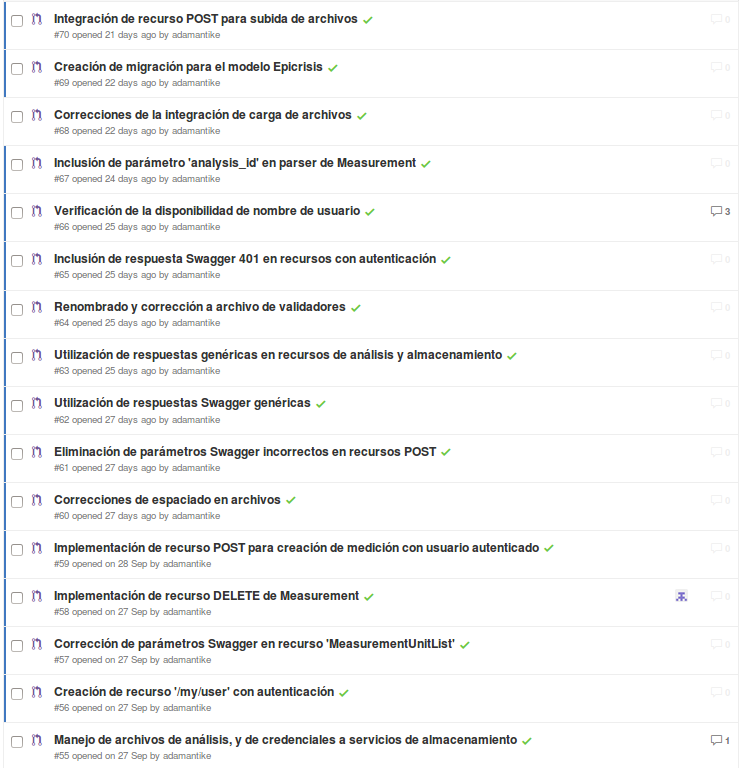
\includegraphics[width=.5\textwidth]{img/6-PR_1}
	\caption{Pull request realizados en el sprint  6}
	\label{6-PR_1}
\end{figure}

\begin{figure}[h!]
	\centering
	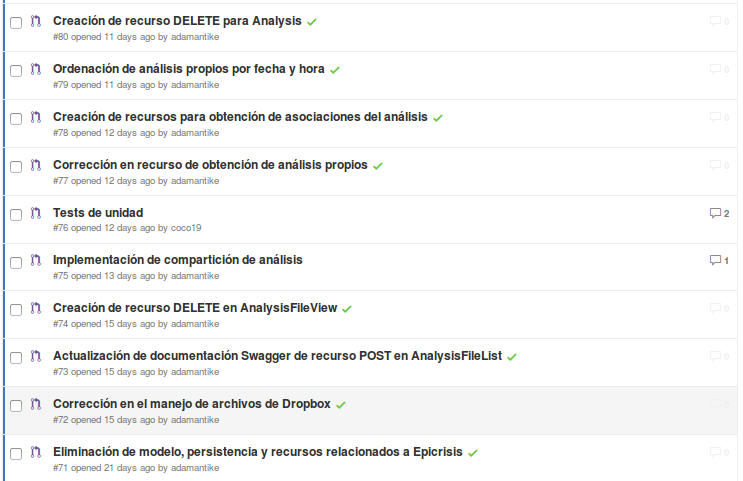
\includegraphics[width=.8\textwidth]{img/6-PR_2}
	\caption{Pull request realizados en el sprint 6}
	\label{6-PR_2}
\end{figure}
\clearpage

\subsection{Modelo funcional} %Diagrama de Casos de uso
A continuación se expone el diagrama de casos de uso del presente Sprint \textbf{[Figura \ref{6-cu}]} acompañado de los casos de uso que se obtuvieron como resultado de los sprint anteriores



\begin{figure}[h]
	\centering
	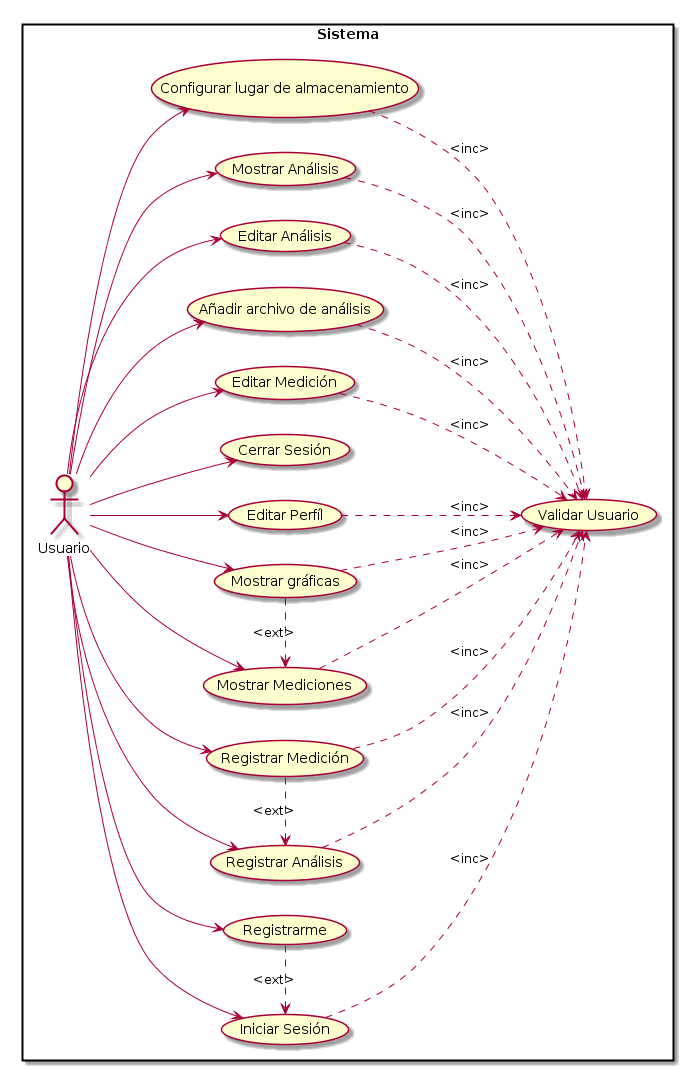
\includegraphics[width=0.6\textwidth]{img/6-cu}
	\caption{formulario de edición de perfil}
	\label{6-cu}
\end{figure}

\clearpage

\subsection{Modelo de datos}
El Diagrama propio de este sprint se puede ver en la \textbf{Figura \ref{5-diagramaClases}}, en ella se indican exactamente las clases que se usarán en este sprint. Estas clases representan un incremento en el diseño de las clases definidas en el sprint 2 de mediciones ya que unifica en un análisis todas las medidas relacionadas evitando la existencia de mediciones colgadas para las cuales no se indica una referencia que denote el motivo de la toma de dicha medición.

    \begin{figure}[h]
        \centering
        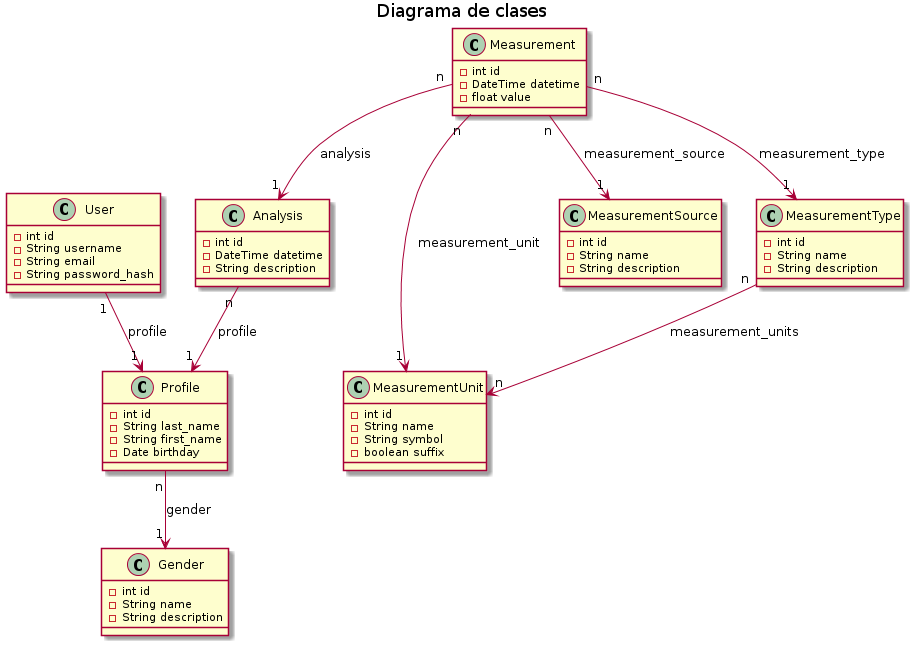
\includegraphics[width=0.8\textwidth]{img/sprint5_dc}
        \caption{Diagrama de clases referido a la carga de análisis}
		\label{5-diagramaClases}
    \end{figure}


\subsection{Diseño}

	Se define el modelo para la gestión de los análisis \textbf{Analysis} el cual presenta los siguientes \textbf{atributos}:

\begin{itemize}
	\item \textbf{id:} Identificador único del modelo.
	\item \textbf{description:} Descripción del análisis.
	\item \textbf{datetime: }	Fecha y hora de creación del análisis.	
	\item \textbf{profile\_id: } Identificador único del perfil al que pertenece el análisis.
\end{itemize}

	Este modelo presenta dos recursos que pueden ser usados por el cliente de la API, los recursos no visibles \textbf{AnalysisList} que ofrece servicios para la carga de nuevos análisis y obtener análisis cargados, \textbf{MyAnalysisList} el cual ofrece servicios para obtener todas los análisis del usuario registrado y cargar un análisis que pertenezca al usuario registrado y no pueda ser consultado por otro y el recurso \textbf{AnalysisMeasurementList} para obtener todas las medidas relacionadas a un análisis. Por otro lado tenemos un recurso visible \textbf{AnalysisView} que ofrece servicios para obtener, modificar y eliminar un análisis específico a partir de un identificador.
	
	
	Acompañando la creación de este nuevo modelo se crearon las representaciones para manejar las solicitudes y armar las respuestas de la API en los paquetes parsers el archivo \textbf{analysis.py} y en el paquete fields la clase \textbf{AnalysisFields}.
	
	Se definieron identificadores de acceso (URLs) para acceder a estos recursos desde un cliente.
		\begin{itemize}
			\item \textbf{/analysis/<int:analysis\_id>}
			\item \textbf{/analysis}
			\item \textbf{/analysis/<int:analysis\_id>/measurements}
			\item \textbf{/my/analyses}
		\end{itemize} 
		
	Por otro lado, se modificó el modelo \textbf{Measurement} para ser asociado a un análisis añadiendo el atributo relacional \textbf{analysis}. Con esta modificación se tuvo que actualizar también servicios y representaciones de los recursos que envuelven éste modelo.
	
	Finalmente se crea una nueva versión del script que carga la base de datos para cargar la tabla que mantiene los datos del análisis.

\clearpage
\subsection {Salidas del Sistema - Incrementos}

Luego de finalizado este user story se obtendrán 5 pantallas que se detallarán a continuación:
\begin{enumerate}
	\item \textbf{Vista para acceder a carga de nueva medición}: \textbf{[Figura \ref{5-boton_nuevo_analisis}]} En la imagen se muestra la forma que tiene el usuario de acceder  a realizar la carga de un análisis.
    	\item \textbf{Crear Análisis}: \textbf{[Figura \ref{5-crear_analisis}]} En la imagen se muestra el formulario que corresponde a un análisis. Por lo general los análisis son un conjunto de mediciones las cuales suelen provenir de un estudio presentada en papel. Por eso en el formulario contemplamos dos campos el de carga de mediciones y el de carga de imágenes que a continuación se detallan.
        	\item \textbf{Carga de mediciones}: \textbf{[Figura \ref{5-cargar_medicion}]} Se le permitirá cargar mediciones que realice en algún momento del día como son peso, altura, grasa corporal y glucosa. Deberá indicar la fuente, tipo, unidad y fecha de la medición. Este formulario es el mismo que el descripto en el\textbf{ Sprint 2.}
    \item \textbf{Carga de imágenes}  \textbf{[Figura  \ref{5-cargar_img} ]} Como se explicó anteriormente se le permite al usuario cargar imágenes correspondiente al estudio/análisis realizado. Cabe destacar en este punto y para los subsiguientes en los cuáles se hace mención de la "carga de archivos",  que el equipo de front end, en este sprint, trabajó con stubs para simular la carga de archivos y así poder utilizarlos con el fin de poder definir la mejor forma de mostrarlos al usuario.

    \item \textbf{Imágenes y mediciones cargadas en el formulario:}  \textbf{[Figura \ref{5-mediciones_cargadas}]} Esta interfaz destaca la funcionalidad de edición, eliminación y vista previa que brinda el formulario.

\end{enumerate}

    
    \begin{figure}[h]
        \centering
        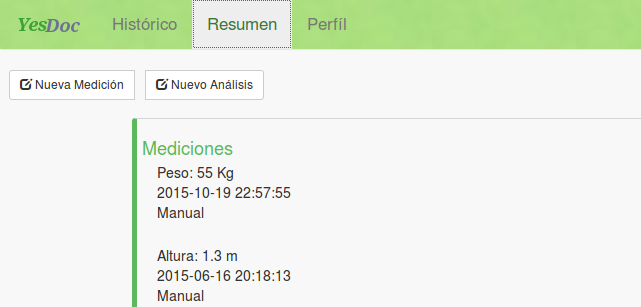
\includegraphics[width=0.5\textwidth]{img/5-boton_nuevo_analisis}
        \caption{vista para acceder a cargar nuevo análisis}
		\label{5-boton_nuevo_analisis}
    \end{figure}
    
    \begin{figure}[h]
        \centering
        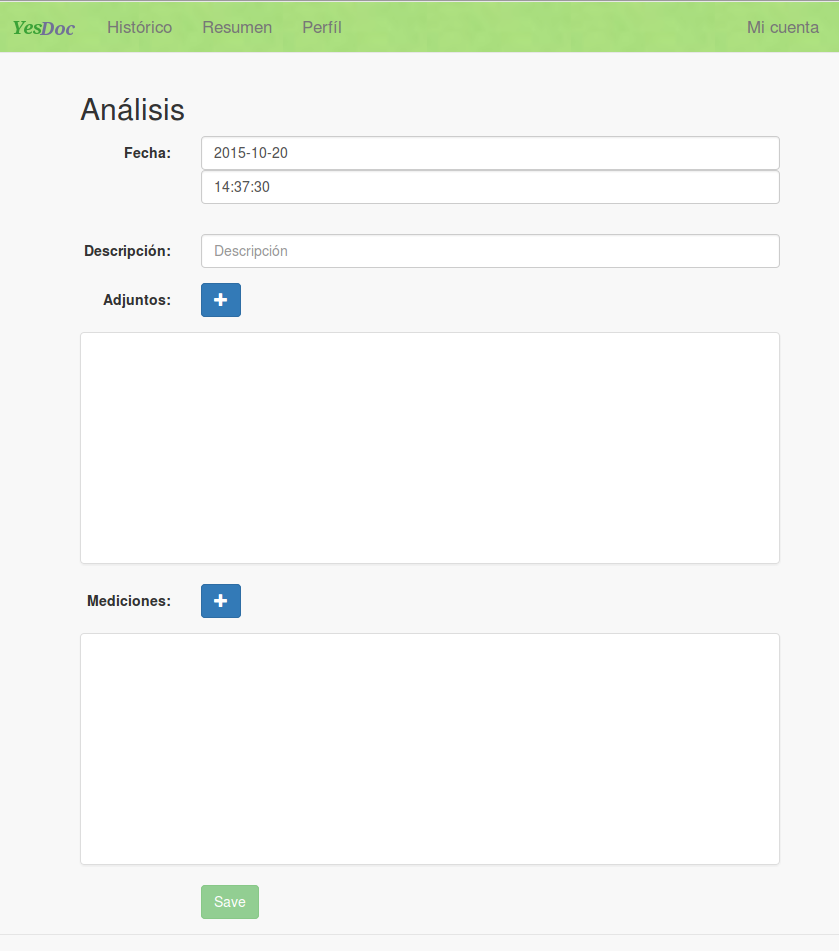
\includegraphics[width=0.5\textwidth]{img/5-crear_analisis}
        \caption{formulario para la creación de análisis}
		\label{5-crear_analisis}
    \end{figure}
    
    \begin{figure}[h]
        \centering
        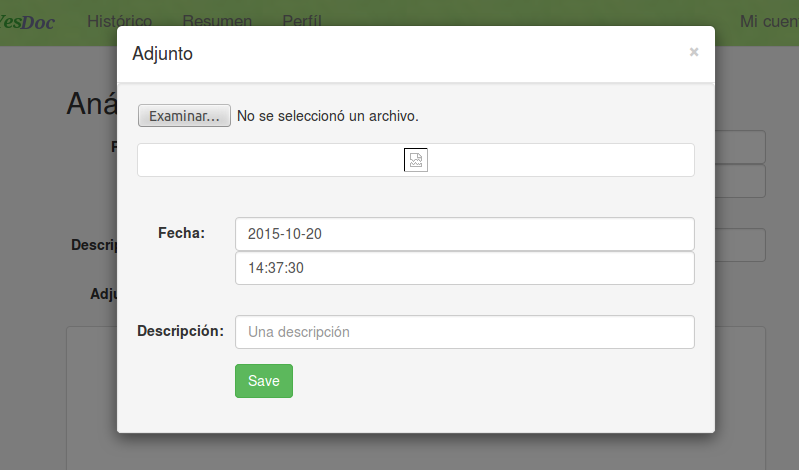
\includegraphics[width=0.5\textwidth]{img/5-cargar_img}
        \caption{formulario de carga de imágenes}
		\label{5-cargar_img}
    \end{figure}
    \begin{figure}[h]
        \centering
        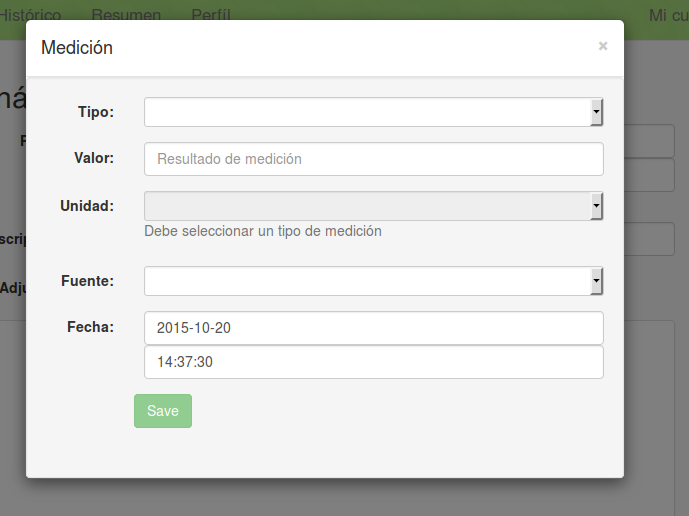
\includegraphics[width=0.5\textwidth]{img/5-cargar_medicion}
        \caption{formulario de carga de medición}
		\label{5-cargar_medicion}
    \end{figure}

    \begin{figure}[h]
        \centering
        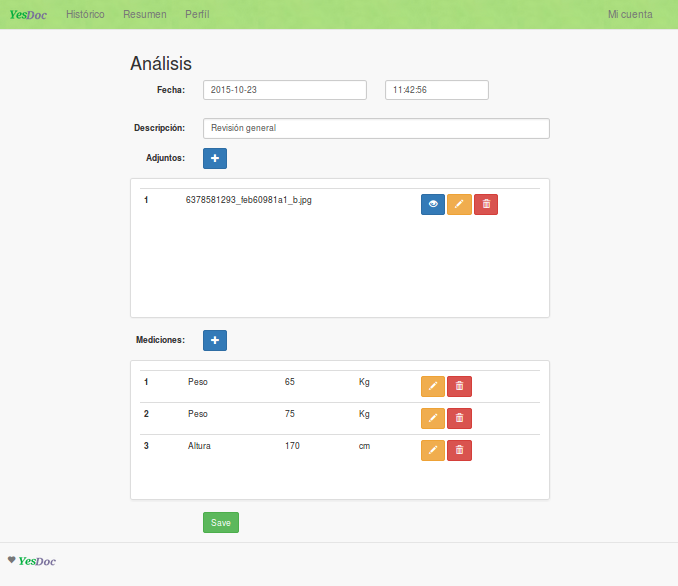
\includegraphics[width=0.5\textwidth]{img/5-mediciones_cargadas}
        \caption{Función de editar, borrar y visualizar}
		\label{5-mediciones_cargadas}
    \end{figure}


\clearpage
\subsection{Planificación y ejecución de pruebas}
\label{s6_planificacion_pruebas}
\subsubsection{Criterios de aceptación}

\begin{center}
\begin{longtable}{|p{0.7cm}|p{4cm}|p{4cm}|p{5cm}| }

	\hline 
		\rowcolor[gray]{0.9} 
		\multicolumn{4}{|c|}{\textbf{Criterio de aceptación}} \\
	\hline
    	\rowcolor[gray]{0.9} 
    	\multicolumn{1}{|c}{\textbf{Id}} & \multicolumn{1}{|c}{\textbf{Contexto}} &  \multicolumn{1}{|c}{\textbf{Evento}} & \multicolumn{1}{|c|}{\textbf{Resultado}} \\
    \hline
    	
1&En caso de que exista una persona sin mediciones & cuando este desee observar sus mediciones  & El sistema no mostrará nada \\ \hline
 
2& Cuando el usuario registrado ingresa dos mediciones del mismo tipo  & y luego quiera consultarlas & El sistema solo le mostrará la ultima medición, del mismo tipo, realizada\\ \hline

3& Cuando el usuario seleccione una medición & y luego quiera editarla & El sistema le permitira la correspondiente edición\\ \hline

4& Si el usuario existe y no está logeado & y quiera ingresar a ver sus mediciones. & El sistema no le permitirá ingresar\\ \hline

5& Si existe al menos un análisis cargado & al solicitar el servicio get del recurso AnalysisList & El sistema retorna una representación en cuyo cuerpo contiene una lista de análisis cargados en el sistema y el código de estado HTTP 200\\ \hline

6& Si existe un perfil cargado con el identificador indicado & l solicitar el servicio get del recurso AnalysisList & El sistema retorna una representación en cuyo cuerpo contiene los datos del análisis cargado en el sistema y el código de estado HTTP 201\\ \hline

7& Si no existe un análisis cargado con el identificador indicado & al solicitar el servicio get del recurso AnalysisView & El sistema retorna una respuesta con código de estado HTTP 404\\ \hline
  \end{longtable}
\end{center}


\subsubsection{Casos de prueba}

\subsubsection{Pruebas  de  integración  entre módulos del Sistema}


\begin{longtable}{|p{4cm}|p{4cm}|p{4cm}|p{3cm}|}
\hline
Actor  & Sistema& Resultado Esperado & Resultado obtenido \\ \hline

El usuario intenta ingresar al sistema & El sistema valida que el usuario con la contraseña ingresada exista 
& Se muestra un cartel de aviso de \textbf{usuario o contraseña invalido} 
& Ok, aunque el cartel podría ser mas vistoso 
\\ \hline



El usuario selecciona \textbf{nuevo perfil}, para
crear una cuenta en YesDoc 
& El sistema direcciona a la vista de creación de perfil
& Muestra formulario de creación de perfil.
&
\\ \hline



 El usuario completa todos los campos y presiona save.
 Ingresa:
\begin{itemize}
	\item \textbf{Nombre de usuario:} Franco
	\item \textbf{Apellido:} Canizo
	\item \textbf{Fecha de nacimiento: }2015-10-90
	\item \textbf{Género: }Masculino
	\item \textbf{Email: }franco@franco
	\item \textbf{pass:}Franco

\end{itemize}
& El sistema anula el botón \textbf{guardar }hasta tanto el usuario cargue todos los campos. una vez cargado todos los campos,al presionar save, redirecciona al menu
de logueo de usuario.
& El sistema informa que ha sido generado su usuario y lo direcciona al formulario de login.
& Ok, pero muestra ciertos mensajes de error al enviar el formulario \textbf{[Issue \#50]}
\\ \hline



El usuario ingresa 
	\textit{\begin{itemize}
		\item \textbf{Nombre de usuario:}Franco
		\item \textbf{Password: }Franco
	\end{itemize} }
&	El sistema valida usuario y contraseña,genera el token, direcciona a myProfileInformation y consulta a la API por la información personal \textbf{Figura \ref{5-login}}
& Se muestra la vista de perfil del usuario indicando sus datos personales
 \begin{itemize}
 		\item \textbf{Nombre de usuario:} Franco 
 		\item \textbf{Apellido: }Canizo 
 		\item \textbf{Fecha de nacimiento: }2015-10-90 
 		\item \textbf{Género: }Masculino
 	\end{itemize}
& Todo Ok, pero podrían aumentarse los colores y quitar espacios en blanco
\\ \hline


Presiona el boton \textit{\textbf{``Editar Perfil'' }}
& El sistema carga la vista \textbf{``profileinformation-edit.html''}, carga la vista correspondiente , valida que el usuario se encuentre logueado pasándole el token que se encuentra almacenado en las cookies. Solicita ala API los datos del perfil y del genero
para rellenar el formulario.
& Se muestra el formulario con los datos del perfil a editar.
& No carga los datos del usuario \textbf{[Issue \#47]}
\\ \hline



Cambia
\textit{
\begin{enumerate}
	\item \textbf{Nombre de usuario :} Franco Nicolás
\end{enumerate}}
&
& Muestra el cambio
& Ok
\\ \hline


Guarda los datos presionando en \textit{\textbf{``guardar''}} 
& El sistema se conecta con la API y guarda los datos a través del método PUT. Redirecciona al perfil de usuario y muestra los datos cambiados
&
Se muestra el perfil con los.
\textit{
\begin{itemize}
	\item \textbf{Nombre de usuario:} Franco Nicolas
	\item \textbf{Apellido:} Canizo
	\item \textbf{Fecha de Nacimiento: }2015-10-90
	\item \textbf{Género:} Masculino
	\item \textbf{Email: }franco@franco
\end{itemize}
}
& Guarda bien, pero al enviar el formulario muestra errores de validación \textbf{[Issue \#50]}
\\ \hline


El usuario presiona en \textbf{``Resumen'' } para ir a la sección donde se muestra una lista de cada medición con su último valor cargado.

& El sistema cambia la url por \textit{\textbf{``\#pro-fileMeasurements''}}, carga la vista correspondiente, valida que el usuario se encuentre logueado pasándole el token que se encuentra almacenado en las cookies y solicita al recurso de la API \textit{\textbf{``my/measurements/latest'' }}las últimas mediciones de cada tipo del usurario. \textbf{Figura \ref{5-perfil}}

& Se muestra una pantalla con dos botones uno para la carga de medición
\textit{\textbf{``Nueva Medición'' }}y otro para la carga de análisis \textit{\textbf{``Nuevo Análisis''}}. No se muestra más datos porque es un usuario nuevo sin información.\textbf{Figura \ref{5-perfil_mediciones}}
& OK
\\ \hline



Selecciona en \textbf{``Nueva análisis'' }
& El sistema direcciona a la url \textit{\textbf{"analy-sis/new"}}, carga la vista correspondiente, valida que el usuario se encuentre logueado pasándole el token que se encuentra almacenado en las cookies.

& Se muestra el formulario de carga de análisis \textbf{[Figura \ref{5-crear_analisis} ]}
& ok
\\ \hline



El usuario carga

\begin{itemize}
	\item \textbf{Fecha :}2015-09-30 16:10:59
	\item \textbf{Descripción: }revisión general
	\item Presionar en .\textbf{``Adjuntos''}

\end{itemize}

&
& El sistema muestra una ventana donde se puede cargar las imágenes con la medición y fecha.\textbf{ [Figura  \ref{5-cargar_img}]}
&ok

\\ \hline



Selecciona una imagen "jpg.o "png", de-ja la fecha igual. 
&
& Se muestra una imagen previa de la imagen. Se muestra la fecha En descripción se muestra el nombre de la imagen
& ok
\\ \hline
 
 

Presiona \textbf{\textit{``guardar''}}
&
& Muestra
\begin{itemize}
	\item Nombre de la descripción de la imagen.
	\item Iconos de visualizar,
	\item \textbf{Iconos de editar}
	\item \textbf{Iconos de borrar.}
\end{itemize}
& ok
\\ \hline





Seleccionar \textit{\textbf{``cargar Medición'' }}
& El sistema se conecta con la API para solicitar tipo y fuentes de mediciones
& El sistema muestra una ventana donde  se puede cargar las mediciones con los siguientes datos:
\textbf{\begin{itemize}
	\item ``Tipo'',
\item ``Valor''
\item ``Unidad''
\item ``Fuente''
\item ``Fecha''
\end{itemize}}
\textbf{[Figura \ref{5-cargar_medicion}]}
& ok
\\ \hline




Selecciona tipo:\textit{\textbf{ "peso"} }
	& El sistema se conecta con la API para
solicitar unidades relacionadas al tipo de medición peso con \textbf{id:``1'' }. \textbf{[Figura \ref{5-crear_medicion}]}
& Muestra las posibles unidades correspondientes al tipo peso
& ok
\\ \hline



Ingresa
\begin{itemize}
	\item \textbf{Tipo:} ``Peso''
	\item \textbf{valor: }``65''
	\item \textbf{Unidad:} ``kilogramo''
	\item \textbf{Fuente: }``manual''
	\item \textbf{Fecha: }``2015:-09-30 16:10:59''
	\item \textbf{ Guardar}
\end{itemize}
&
& Mantiene la misma venta abierta y muestra un mensaje de aviso de que la
medición fue cargada con éxito.\textit{ \textbf{"Bien hecho se cargo una medición''}}
& ok, si bien es útil que mantenga los datos para facilitar la nueva carga, sería conveniente acentuar el aviso de que la medición ya se cargo.
\\ \hline





Modificado el valor ingresado con anterioridad

\begin{itemize}
	\item \textbf{Tipo:} ``Peso''
	\item \textbf{valor: }``75''
	\item \textbf{Unidad:} ``kilogramo".
	\item \textbf{Fuente: }``manual"
	\item \textbf{Fecha: }2015:-10-10 16:10:59
	\item \textbf{ Guardar}
\end{itemize}
&
& Mantiene la misma venta abierta y muestra un mensaje de aviso de que la
medición fue cargada con éxito.\textbf{``Bien hecho se cargo una medición''}
& ok
\\ \hline




Selecciona



\begin{itemize}
	\item \textbf{Tipo:} ``altura'', modifica el valor ingresado con anterioridad
	por
	\item \textbf{valor: }``170''
	\item \textbf{Unidad:} ``centímetro".
	\item \textbf{Fuente: }``manual"
	\item \textbf{Fecha: }2015:-10-23 16:10:59
	\item \textbf{ Guardar}
\end{itemize}
&
&
Mantiene la misma venta abierta y muestra un mensaje de aviso de que
la medición fue cargada con éxito.\textit{\textbf{ ``Bien hecho se cargo una medición''}}
& ok
\\ \hline




Se selecciona el botón \textbf{"guardar"}
& El sistema consulta el perfil a la API para extraer el id el cual se usara para crear un análisis. Envía por POST a la API el análisis y realiza tres llamados mas a la API uno por cada medición cargada.
Mantiene la misma venta abierta y muestra un mensaje de aviso de que
la medición fue cargada con éxito. Almacena en la API el path y el storage\_location de la imagen.Luego direcciona la página a la url
\textit{\textbf{\#/profileMeasurements}}, valida que el token se encuentre activo, si no hay
errores solicita a la API las ultimas mediciones y muestra las mediciones

& En la vista de perfil de mediciones,Lista las últimas mediciones cargadas,
mostrando el peso cargado mas recientemente

\begin{itemize}
	\item Peso: 65 Kg Fecha 2015-10-2314:42:56 Manual
	\item Altura: 170 cm 2015-10-2314:42:56 Manual

\end{itemize}
& ok, habría que explicar que para ver todos sus pesos debería dirigirse a histórico

\\ \hline






Selecciona el icono de edición ubicado al lado de la medición \textit{Peso 65Kg}
& El sistema redirecciona \textbf{\#/measure-ments/103/edit}, verifica con la API que el token se encuentre activo, a partir del\textbf{ id} de la medición seleccionada para editar trae de la API el \textbf{tipo de medición, el valor, la unidad, la fuente y la fecha.}

& Se muestra un formulario con los datos de la medición precargadas
\begin{itemize}
	\item \textbf{Tipo:}Peso 
	\item \textbf{Valor: }65 
	\item \textbf{Unidad:} kilogramo
	\item \textbf{Fuente:}Manual 
	\item \textbf{Fecha:}2015-10-23 -14:42:56
\end{itemize}
&  ok
\\ \hline





Cambia la \textit{\textbf{fecha y la hora} por 2015-5-13- 4:42:56 }y guarda los cambios.
& El sistema guarda la medición, redirecciona\textbf{ \#/profileMeasurements }valida el token, y solicita las últimas mediciones a la API

& Muestra la interfaz con las últimas mediciones 
\begin{itemize}
	\item Peso: 75 Kg 2015-10-23 14:42:56 Manual 
	\item Altura: 170 cm 2015-10-23 14:42:56 Manual
\end{itemize}
& ok
\\ \hline





El usuario selecciona en \textit{\textbf{nueva medición}}
& El sistema redirecciona a \textbf{\#/measure-ments/new} valida contra la API que el Token se encuentra activo, luego trae los tipos de mediciones

& Muestra el formulario para cargar una medición con los siguientes valores 
\textbf{\begin{itemize}
	\item Tipo: 
	\item Valor:
	\item  Unidad: 
	\item Fuente: 
	\item Fecha:
\end{itemize}}
& ok
\\ \hline






El usuario selecciona en \textbf{``nueva medición''} 
\begin{itemize}
	\item \textbf{Tipo:}Peso
	\item \textbf{ Valor: }70
	\item\textbf{ Unidad:}-kilogramo
	\item \textbf{Fuente:}Manual
	\item \textbf{ Fecha:}2015-19-23 -14:42:56 
	\item \textbf{Guardar}
\end{itemize}

& El sistema redirecciona a \textbf{\#/profile-Measurementsvalida }contra la API que el Token se encuentra activo y luego trae las últimas mediciones

& Muestra la lista de últimas mediciones
\textbf{\begin{itemize}
	\item Peso: 75 Kg 2015-10-23 14:42:56 Manual
	\item Altura: 170 cm 2015-10-23 14:42:56 Ma-nual
\end{itemize}}
& ok
\\ \hline




Presionar en sección \textbf{``histórico''}
& El sistema redirecciona a\textbf{ \#/home }y se carga la vista correspondiente a  \textbf{  weight,} se verifica que el token este activo, se traen todas las medidas de tipo peso
& Se muestra una botonera con los tipos de mediciones , una gráfica y una tabla con las 3 medidas de tipo \textbf{Peso}
& ok, la botonera debería ser horizontal
\\ \hline




Presionar en sección \textbf{Altura }
& El sistema carga la vista correspondiente a height, se verifica que el token este activo, se traen todas las medidas de tipo peso
& Se muestra una botonera con los tipos de mediciones , una gráfica y una tabla con una medida \textbf{170 centímetros} de la altura.
& ok
\\ \hline





Presionar en sección \textit{\textbf{Análisis }} 
& El sistema carga la vista correspondiente a análisis, se verifica que el token este activo, se traen los análisis de la API
& Se muestra el análisis cargado con anterioridad mostrando la imagen, la descripción y la fecha seleccionada por el usuario.
& ok
\\ \hline






Selecciona el \textit{\textbf{Análisis}}
& El sistema carga la vista correspondiente a \textbf{ \#/home/analyses}, se verifica que el token este activo, trae los datos y los archivos del análisis de la API
& Se muestran las imágenes (en este caso sólo una) y una tabla con las mediciones de ese análisis.
& Falla en chrome, no muestra las imágenes
\\ \hline




Selecciona \textit{\textbf{Mi cuenta}}, luego \textit{\textbf{Cerrar Sesión}}
& El sistema direcciona \textbf{\#/logoof } y da de baja el token
& Se muestra la interface de login
& ok
\\ \hline


\end{longtable}







    \begin{figure}[h]
        \centering
        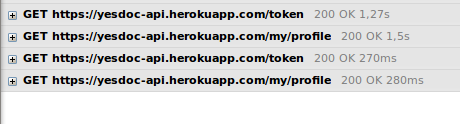
\includegraphics[width=0.5\textwidth]{img/5-login}
        \caption{Respuesta de la API al loguearse}
		\label{5-login}
    \end{figure}
    
        \begin{figure}[h]
        \centering
        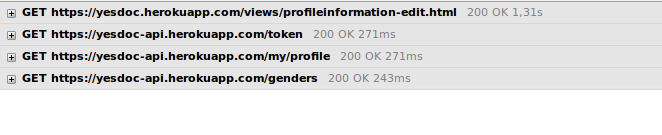
\includegraphics[width=0.5\textwidth]{img/5-perfil}
        \caption{Respuesta de la API al mostrar perfil}
		\label{5-perfil}
    \end{figure}
    
        \begin{figure}[h]
        \centering
        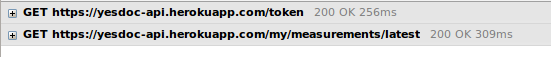
\includegraphics[width=0.5\textwidth]{img/5-resumen}
        \caption{Respuesta de la API al mostrar últimas mediciones}
		\label{5-resumen}
    \end{figure}
    
    \begin{figure}[h]
        \centering
        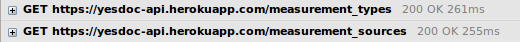
\includegraphics[width=0.5\textwidth]{img/5-crear_medicion}
        \caption{Respuesta de la API al crear nuevo análisis}
		\label{5-crear_medicion}
    \end{figure}
    
    
    
    
    \begin{figure}[h]
        \centering
        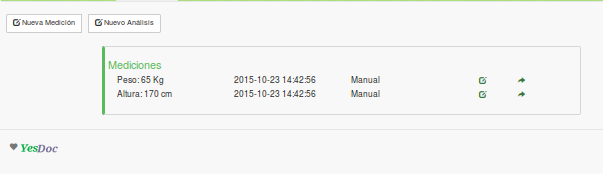
\includegraphics[width=0.5\textwidth]{img/5-perfil_mediciones}
        \caption{Perfil de mediciones}
		\label{5-perfil_mediciones}
    \end{figure}
    
    \begin{figure}[h]
        \centering
        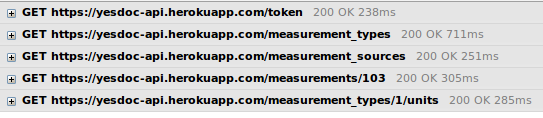
\includegraphics[width=0.5\textwidth]{img/5-editar_medicion}
        \caption{Respuesta de la API al editar mediciones}
		\label{5-editar_medicion}
    \end{figure}
    
    \begin{figure}[h]
        \centering
        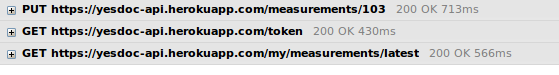
\includegraphics[width=0.5\textwidth]{img/5-fin_editar_medicion}
        \caption{Respuesta de la API al editar nuevo análisis}
		\label{5-fin_editar_medicion}
    \end{figure}
    
    \begin{figure}[h]
        \centering
        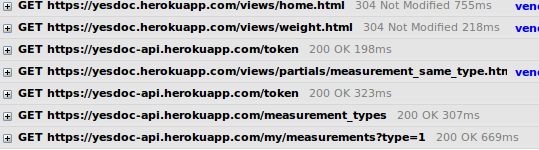
\includegraphics[width=0.5\textwidth]{img/5-mostrar_grafica}
        \caption{Respuesta de la API al mostrar gráficas}
		\label{5-mostrar_grafica}
    \end{figure}
    
    \begin{figure}[h]
        \centering
        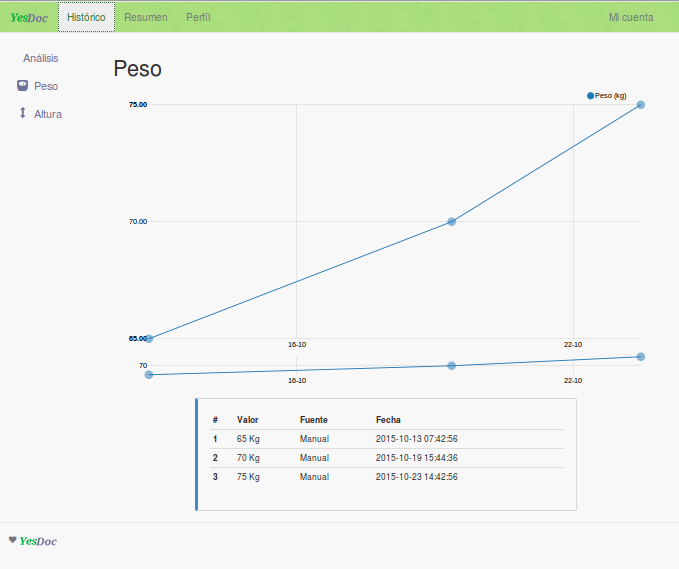
\includegraphics[width=0.5\textwidth]{img/5-grafica_medicion}
        \caption{Vista de gráfica y tablas de mediciones}
		\label{5-curva_medicion}
    \end{figure}
    
    \begin{figure}[h]
        \centering
        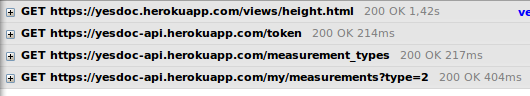
\includegraphics[width=0.5\textwidth]{img/5-grafica_altura}
        \caption{Respuesta de la API al mostrar la gráfica de altura}
		\label{5-grafica_altura}
    \end{figure}
    
    \begin{figure}[h]
        \centering
        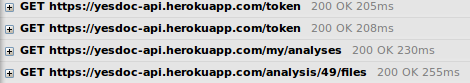
\includegraphics[width=0.5\textwidth]{img/5-mostrar_analisis}
        \caption{Respuesta de la API al mostrar los análisis}
		\label{5-mostrar_analisis}
    \end{figure}
    
    \begin{figure}[h]
        \centering
        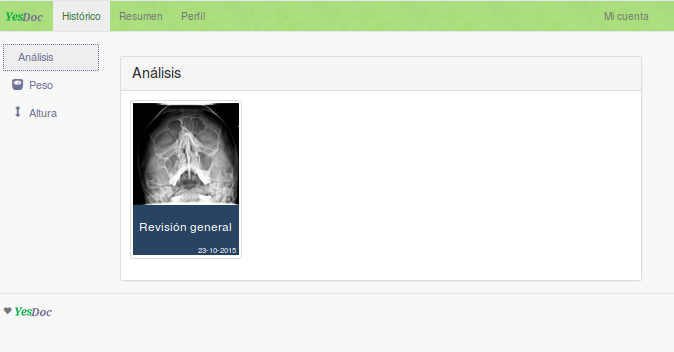
\includegraphics[width=0.5\textwidth]{img/5-mostrar_analisis_pag}
        \caption{Vista de la lista de análisis}
		\label{5-mostrar_analisis_pag}
    \end{figure}
    
    \begin{figure}[h]
        \centering
        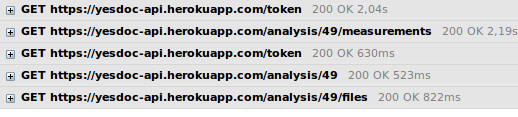
\includegraphics[width=0.5\textwidth]{img/5-analisis}
        \caption{Respuesta de la API al consultar los análisis}
		\label{5-analisis}
    \end{figure}
    
    \begin{figure}[h]
        \centering
        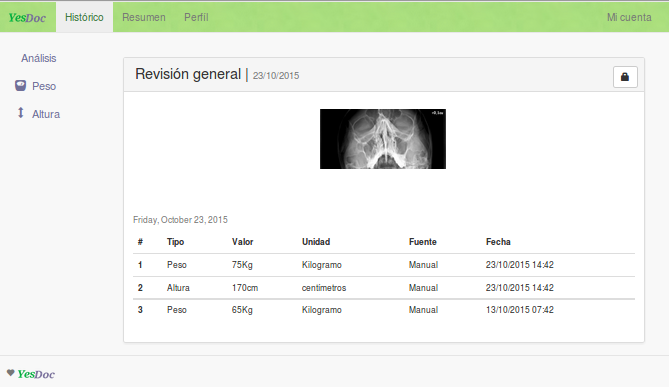
\includegraphics[width=0.5\textwidth]{img/5-contenido_analisis}
        \caption{Vista del contenido del análisis}
		\label{5-contenido_analisis}
    \end{figure}
    
    \begin{figure}[h]
        \centering
        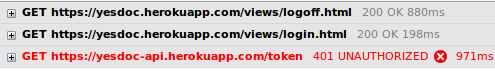
\includegraphics[width=0.5\textwidth]{img/5-logoff}
        \caption{Respuesta de la API al cerrar sesión}
		\label{5-logoff}
    \end{figure}
    



\clearpage



\subsubsection{Pruebas de carga}
Se va a simular el acceso a la página hosteada en Heroku, de un lote de usuarios. Además en la gráfica \textbf{[Figura \ref{prueba_carga_50_us}]}se puede ver los tiempos de respuesta al ir incrementando la cantidad de usuarios.

\begin{center}
\begin{tabular}{|c|c|}
	\hline Cantidad de Usuario  &  Tiempo de espera\\ 
	\hline 20 usuarios &  155 ms \\ 
	\hline 30 usuarios  & 115 ms \\ 
	\hline 40 usuarios  & 100 ms \\ 
	\hline 50 usuarios  & 130 ms \\ 	
	\hline 
\end{tabular} 
\end{center}

    \begin{figure}[h]
    	\centering
    	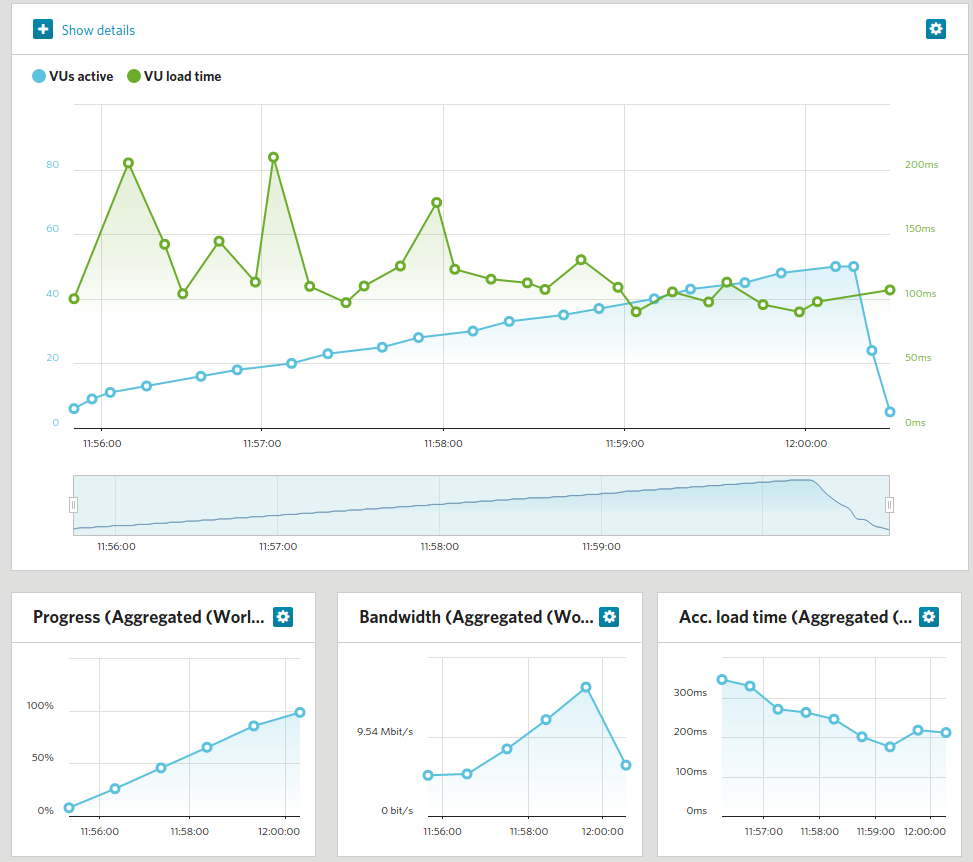
\includegraphics[width=0.5\textwidth]{img/prueba_carga_50_us}
    	\caption{Prueba de carga simulando 50 usuarios}
    	\label{prueba_carga_50_us}
    \end{figure}


\subsubsection{Pruebas de performance}
Google developers mide de 0 a 100 la velocidad de carga del sitio e indica, por orden de prioridad, qué mejorar, aportando información al respecto.
en nuestro caso nos recomienda disminuir el tamaño de las imágenes \textbf{[Figura \ref{prueba_velocidad_1}]}

\newpage

    \begin{figure}[h]
    	\centering
    	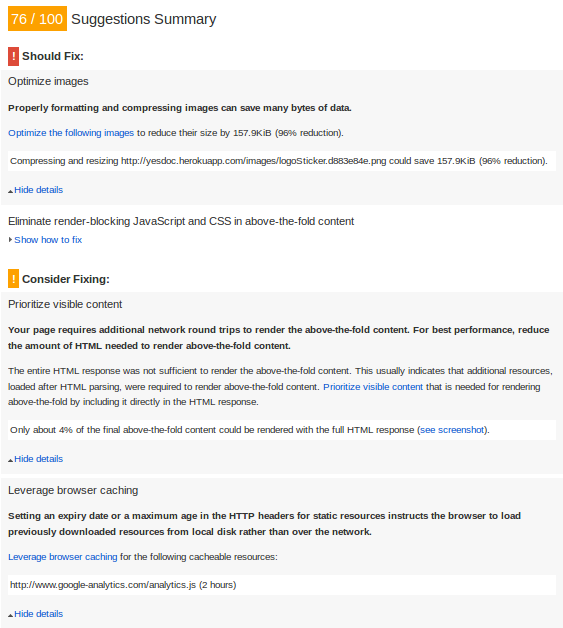
\includegraphics[width=0.5\textwidth]{img/prueba_velocidad_1}
    	\caption{Pruebas de velocidad en desktop}
    	\label{prueba_velocidad_1}
    \end{figure}

    \begin{figure}[h]
    	\centering
    	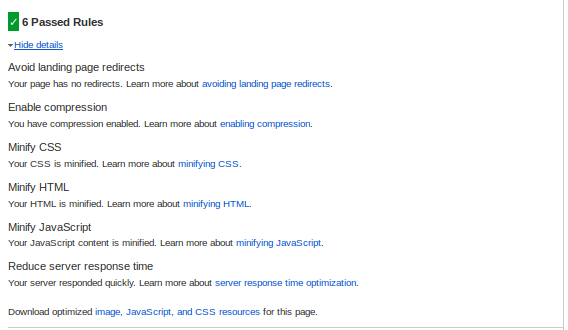
\includegraphics[width=0.5\textwidth]{img/prueba_velocidad_2}
    	\caption{Pruebas de velocidad pasadas}
    	\label{prueba_velocidad_2}
    \end{figure}

\newpage

\begin{longtable}{|p{1.0cm}|p{3cm}|p{3cm}|p{3.5cm}|p{2.5cm}|}
	\hline \hline
		\rowcolor[gray]{0.9} 
		\multicolumn{1}{|c}{ID} & \multicolumn{1}{|c|}{Descripción} & \multicolumn{1}{c|}{Precondiciones} & \multicolumn{1}{c|}{Pasos} &
		\multicolumn{1}{c|}{Resultado} \\
	\hline
	PC-1 & Se cargan 100 análisis a 5 perfiles  & Existen precargados instancias de Profile y Gender & Se generan instancias de Gender (Masculino y Femenino) y se generan 5 instancias de perfiles de usuarios diferentes, se hacen peticiones HTTP con método post al servicio \textbf{/analysis} & \textbf{Figura \ref{pc_a_1}} \\
	\hline
	PC-2 & Se obtienen 100 análisis de 5 perfiles & Existen precargados 100 análisis & Se cargan 100 análisis, se hace una petición http utilizando el método get al servicio \textbf{/analysis} & \textbf{Figura \ref{pc_a_2}}\\
		\hline

\end{longtable}

\begin{figure}[h]
    \centering
    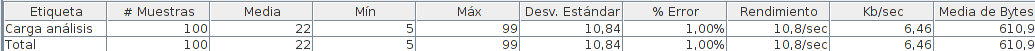
\includegraphics[width=0.85\textwidth]{img/PC_analisis_1}
    \caption{Resultado prueba de carga de 100 análisis.}
	\label{pc_a_1}
\end{figure}

\begin{figure}[h]
    \centering
    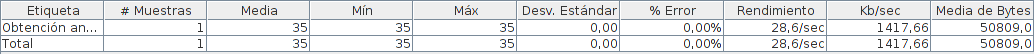
\includegraphics[width=0.85\textwidth]{img/PC_analisis_2}
    \caption{Resultado prueba de obtención de 100 análisis.}
	\label{pc_a_2}
\end{figure}
\clearpage
\subsubsection{Pruebas de seguridad por niveles de usuarios}

\begin{longtable}{|p{1.0cm}|p{4cm}|p{4cm}|p{4cm}| }

	\hline
		\rowcolor[gray]{0.9} 
		\multicolumn{1}{|c}{Id test seguridad} & \multicolumn{1}{|c|}{Contexto} & \multicolumn{1}{|c|}{Evento} & \multicolumn{1}{|c|}{Resultado esperado} \\
	\hline
		ST-1 & Si el token utilizado en el header Authorization de la solicitud no corresponde a un usuario del sistema  & al solicitar el servicio put del recurso AnalysisView & El sistema retorna una respuesta con código de estado HTTP 401, UNAUTHORIZED\\
	\hline
		ST-2 & Si el token utilizado en el header Authorization de la solicitud corresponde a un usuario del sistema pero no al usuario al que pertenece el analysis & al solicitar el servicio put del recurso AnalysisView & El sistema retorna una respuesta con código de estado HTTP 403, FORBIDDEN\\
	\hline
		ST-3 & Si el token utilizado en el header Authorization de la solicitud corresponde a un usuario del sistema, el análisis con el identificador existe y el token pertenece al usuario al que pertenece el análisis & al solicitar el servicio put del recurso AnalysisView & El sistema retorna en el cuerpo de la respuesta los datos del análisis y el código de estado HTTP 200, UPDATED\\
	\hline
		ST-4 & Si el token utilizado en el header Authorization de la solicitud corresponde a un usuario del sistema, el análisis con el identificador existe y el token pertenece al usuario al que pertenece el análisis & al solicitar el servicio delete del recurso AnalysisView & El sistema retorna la respuesta con código de estado HTTP 204, DELETED\\
	\hline

\end{longtable}

\subsection{Retroalimentación de pruebas}
	\begin{itemize}
		\item \textbf{¿Qué fue bien?}
        	\begin{itemize}
				\item La carga de análisis, junto a las mediciones e imágenes funciona correctamente
				\item Listar los análisis y su contenido funcionan bien en Firefox.
				\item Se definió correctamente la gestión de análisis y el uso de autenticación para la gestión de análisis personales.
				\item Se armaron las vistas que permiten al usuario crear análisis y cargar mediciones e imágenes a los mismos.
			\end{itemize}
		\item \textbf{¿Qué fue mal?}
		\begin{itemize}
			\item \textbf{Abierto} Las imágenes de los análisis no es posible verlo en el navegador Chrome.
			
		\end{itemize}
   		\item \textbf{¿Qué se mejoró?}
        	\begin{itemize}
                \item \textbf{Cerrado} Los colores e imágenes de los botones.
                \item \textbf{Cerrado} Se permite hacer zoom en las gráficas.
                \item Se mejoró la captura de mediciones permitiendo que estas se engloben en el contexto de un análisis lo cual les da una razón de ser.
			\end{itemize}

   		\item \textbf{¿Qué se puede mejorar?}
        	\begin{itemize}
		       \item \textbf{Abierto} La posición de la botonera en la sección histórico no es la correcta.
		       \item \textbf{Abierto}  El aviso de medición cargada debería ser mas nítido.
		       \item \textbf{Abierto} Al cargar un nuevo usuario y al modificarlo, el formulario muestra errores, esto produce desconcierto en el usuario.
		        \item Se debe mejorar en cuanto a los tiempos de trabajo del back end para brindar soluciones que puedan ser usadas a tiempo por el front end.
		        \item En cuanto a la gestión de análisis se podría definir que cuando el usuario cargue su primer medida del día, sin indicar un análisis específico, se cree automáticamente un análisis con descripción ``Análisis diario'' si es que éste aún no existe.
            \end{itemize}
        

	\end{itemize}